\documentclass{beamer}
\usepackage[latin1]{inputenc}
\usetheme{Goettingen}
\title[SDF Crash Course]{Synchronous Dataflow\\A Crash Course in Infinite Programs}
\author{Nic Hollingum}
\institute{USYD}
\date{7 Apr, 2011}
\begin{document}

\begin{frame}
\titlepage
\end{frame}

%BACKGROUND INFO
\section{Background}

\begin{frame}{Problem}
\begin{columns}
\begin{column}{6cm}
\begin{itemize}
	\item Not all programs are suited to traditional Von-Neuman model
	\item Digital Signal Processing
	\item Programming these devices is difficult\cite{lee87}
	\item Represent this kind of computation more naturally
\end{itemize}
\end{column}
\begin{column}{4cm}
\center{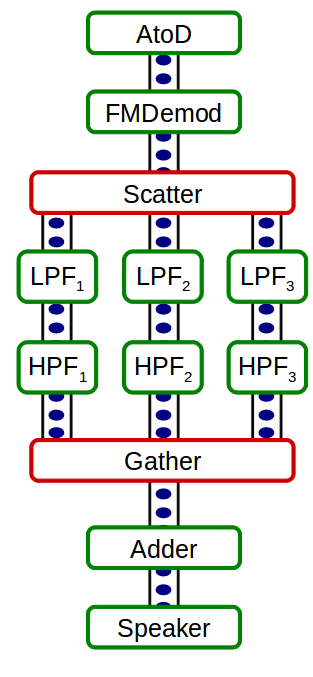
\includegraphics[height=7cm]{../res/multiradio.png}}
\end{column}
\end{columns}
\end{frame}

\begin{frame}{Solution}
\begin{itemize}
	\item Termination is ill-defined, programs can run for infinity
	\item Expressive notion of data rates
	\item Control via sequencing of data - ties inputs to outputs
	\item hence Synchronous Dataflow
\end{itemize}
\end{frame}


%REPRESENTING A STREAM GRAPH
\section{Representation}

\begin{frame}{Tokens}
\begin{columns}
\begin{column}{5cm}
\begin{itemize}
	\item Single unit of data
	\item Data Streams represented by sequences of tokens
	\item Discreet, but vary in size
	\item Some tokens are provided by user at execution, others arrive as input
	\item Data-rates of tokens must be known at compile time
\end{itemize}
\end{column}
\begin{column}{5cm}
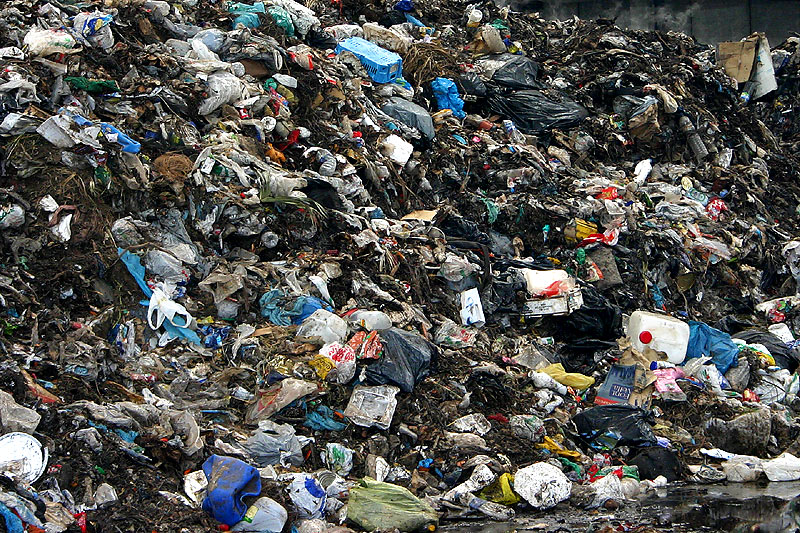
\includegraphics[width=5cm]{../res/pile-of-garbage.jpg}
\end{column}
\end{columns}
\end{frame}

\begin{frame}{Channels}
\begin{columns}
\begin{column}{5cm}
\begin{itemize}
	\item Paths along which tokens flow
	\item Simple FIFO buffers
	\item Connect data between computational units (network)
\end{itemize}
\end{column}
\begin{column}{5cm}
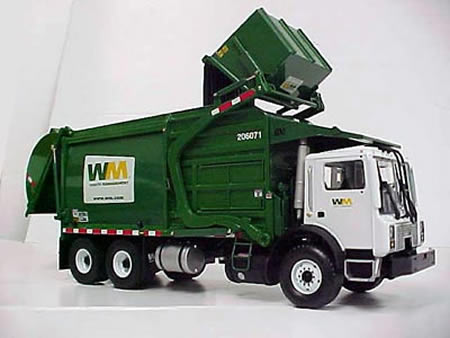
\includegraphics[width=5cm]{../res/waste-management-truck.jpg}
\end{column}
\end{columns}
\end{frame}

\begin{frame}{Actors}

\begin{columns}
\begin{column}{6cm}
\begin{itemize}
	\item individual computation units
	\begin{itemize}
		\item Simple: 2 $\rightarrow$ add $\rightarrow$ 1
		\item Complicated: $2^n$ $\rightarrow$ FFT $\rightarrow$ $2^n$
	\end{itemize}
	\item Consumes a number of tokens on input channels and produces on others
	\item ammount consumed need not equal ammoun produced by predecessor
	\begin{itemize}
		\item Must be known at compile time
		\item Possibly cosumes and produces from the same channel (feedback)
	\end{itemize}
	\item Stateful or Stateless
\end{itemize}
\end{column}
\begin{column}{4cm}
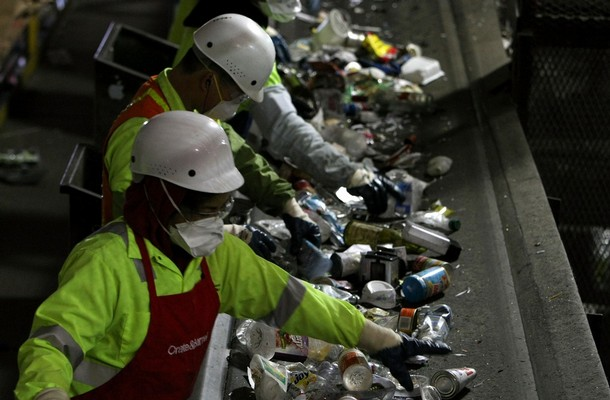
\includegraphics[width=4cm]{../res/sf-recycling-center.jpg}
\end{column}
\end{columns}
\end{frame}

\begin{frame}{Delays}
\begin{columns}
\begin{column}{5cm}
\begin{itemize}
	\item Signal processing kinds of delays
	\item Allows feedback loops to be non-terminating
	\item Working out the required delays is possible though not easy
\end{itemize}
\end{column}
\begin{column}{5cm}
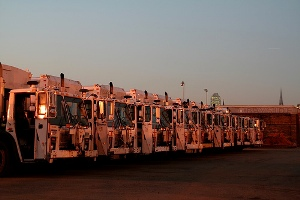
\includegraphics[width=5cm]{../res/2007_10_garbtrucks.jpg}
\end{column}
\end{columns}
\end{frame}

\begin{frame}{SDF Graphs}
\begin{itemize}
	\item Graphical representation of SDF network
	\item Actors are vertices
	\item Channels are Arcs
	\item Arcs are annotated with Delays and Consumption/production
\end{itemize}
\end{frame}


\begin{frame}{SDF Graphs}
\begin{center}
	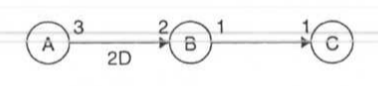
\includegraphics[width=8cm]{../res/simplesdf.png}

	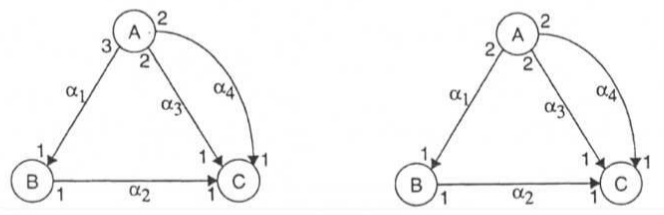
\includegraphics[width=8cm]{../res/validinvalid.png}

	\cite{sdfbook}
\end{center}
\end{frame}

%TOPOLOGY MATRIX AND ITS PROPERTIES
\section{Tolopogies}

\begin{frame}{Topology Matrix}\
\begin{itemize}
	\item Graph: $\Gamma = \mathbb{R}^{|L| \times |A|}$
	\item A row for each link and a column for each actor
\end{itemize}

\[
  \Gamma_{l, a} = \left\{
  \begin{array}{l l}
    0 & \quad \text{if $a$ is not an endpoint of $l$}\\
    prod(l) & \quad \text{if $a$ is the start-point of $l$}\\
    -cons(l) & \quad \text{if $a$ is the end-point of $l$}
  \end{array} \right.
\]\
\end{frame}

\begin{frame}{Topology Matrix}\
\[
 \Gamma = \begin{bmatrix}
	1 & -1 & 0 & 0 & 0 & 0 & 0 \\
	0 & 2 & -1 & 0 & 0 & 0 & 0 \\
	0 & -2 & 1 & 0 & 0 & 0 & 0 \\
	0 & 1 & 0 & -1 & 0 & 0 & 0 \\
	0 & 0 & 3 & 0 & -2 & 0 & 0 \\
	0 & 0 & 0 & 0 & 1 & -2 & 0 \\
	0 & 0 & 0 & 3 & 0 & -2 & 0 \\
	0 & 0 & 0 & 4 & 0 & 0 & -3 \\
	0 & 0 & 0 & 0 & 0 & 8 & -9 \\
     \end{bmatrix}
\]
\end{frame}

%SOME NAIVE SCHEDULING
\section{Scheduling}

\begin{frame}{Repetitions Vector}
\begin{columns}
\begin{column}{5cm}
\begin{itemize}
	\item Topology matrix used to schedule actors
	\item Repetitions Vector is an invocation of actors counter
	\item if every actor is invoked as many times as the RV says, the number of tokens after the execution(s) is the same as before
	\begin{itemize}
		\item i.e. $\Gamma \mathbf{r} = \mathbf{0}$
	\end{itemize}
	\item called ``steady state''
\end{itemize}
\end{column}
\begin{column}{5cm}
\begin{center}
\[
\begin{bmatrix}
	6\\
	6\\
	12\\
	6\\
	18\\
	9\\
	8\\
\end{bmatrix}
\]
\end{center}
\end{column}
\end{columns}
\end{frame}

\begin{frame}{Schedules}
\begin{block}{Pediodic Schedule}
A list of actor invocations that return to the steady state
\end{block}
\pause
\begin{block}{Init Schedule}
A list of actor invocations that flood the buffers to the desired level
\end{block}
\pause
\begin{block}{``Death Schedule''}
A list of actor invocations that drain the buffers to the initial level (i.e. with the given delays)
\end{block}
\end{frame}

\begin{frame}{Periodic}
\begin{columns}
\begin{column}{5cm}
\begin{itemize}
	\item Execution order doesnt affect fill state
	\item May require prohibitively large buffers
	\item Cant execute if we dont have data in the buffers
	\item we can fiddle with the order to reduce buffer size (NP-Hard)
\end{itemize}
\end{column}
\begin{column}{5cm}

\includegraphics[width=5cm]{../res/recycle.jpg}
\end{column}
\end{columns}
\end{frame}

\begin{frame}{Init and Death}
\begin{columns}
\begin{column}{6cm}
\begin{itemize}
	\item Fills and clears the buffers
	\item We have to know in advance how much we want to fill the buffers
	\item It may be a good idea to fill so that {\bf any} periodic schedule may execute
	\item presume all actors simultaneously execute all their repetitions at the start
	\item delay actor invocations if we know buffers wont be full.
	\begin{itemize}
		\item Strategically place actors
		\item avoid costly dynamic scheduling
	\end{itemize}
\end{itemize}
\end{column}
\begin{column}{4cm}
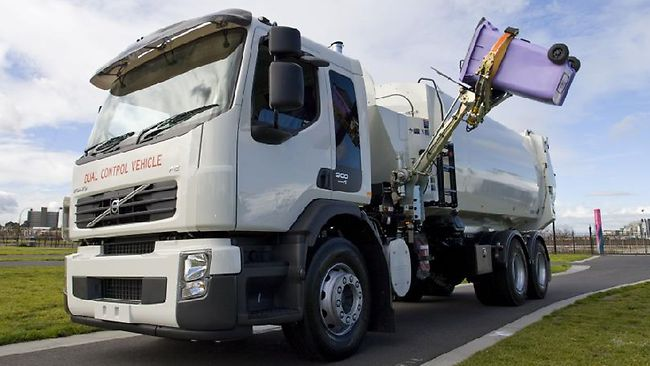
\includegraphics[width=4cm]{../res/garbage-in.jpg}

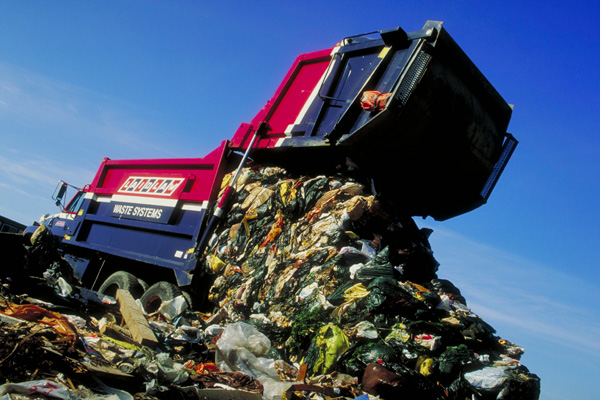
\includegraphics[width=4cm]{../res/GarbageOut.jpg}
\end{column}
\end{columns}
\end{frame}

%MY RESEARCH FOCUS
\section{My Research}

\begin{frame}{Cloud Applications}
\begin{itemize}
	\item massive virtual machines/multiple virtual machines
	\item network bandwidth is an important consideration
	\item small probability of node failure, whole computation is gone
	\item develop schemes to ensure fault tolerance
	\begin{itemize}
		\item Statically replicate multiple nodes
		\item Dynamically re-compute if a node fails
	\end{itemize}
	\item examine trade-off between Makespan, Network Cost, and Fault tolerance
\end{itemize}
\end{frame}

\begin{frame}{N-Process Machines}
\begin{itemize}
	\item abstraction from (single-core/multi-core/multi-processor/cloud) machines
	\item Use cost matrices to account for varying bandwith/processing capabilities
	\begin{itemize}
		\item 2 cores in the same machine have 0 communication cost
		\item Actors assigned to a 1ghz processor take longer than those on a 1.8ghz processor
	\end{itemize}
	\item Use this machine specification to generate a mapping of actors to processors
	\item Most must be approximated, optimality is NP-Hard
\end{itemize}
\end{frame}

%TIDYING UP
\section{References}
\begin{frame}[allowframebreaks]{References}
\bibliographystyle{wmaainf}
\bibliography{biblio}
\end{frame}

\end{document}
